\documentclass{article}

% if you need to pass options to natbib, use, e.g.:
% \PassOptionsToPackage{numbers, compress}{natbib}
% before loading nips_2018

% ready for submission
%\usepackage{nips_2018}

% to compile a preprint version, e.g., for submission to arXiv, add
% add the [preprint] option:
\usepackage[preprint]{nips_2018}

% to compile a camera-ready version, add the [final] option, e.g.:
% \usepackage[final]{nips_2018}

% to avoid loading the natbib package, add option nonatbib:
% \usepackage[nonatbib]{nips_2018}

\usepackage[utf8]{inputenc} % allow utf-8 input
\usepackage[T1]{fontenc}    % use 8-bit T1 fonts
\usepackage{hyperref}       % hyperlinks
\usepackage{url}            % simple URL typesetting
\usepackage{booktabs}       % professional-quality tables
\usepackage{amsfonts}       % blackboard math symbols
\usepackage{nicefrac}       % compact symbols for 1/2, etc.
\usepackage{microtype}      % microtypography
\usepackage{amsmath}
\usepackage{amsthm}
\usepackage{enumerate}
\usepackage{comment}
\usepackage{url}
\usepackage{amsfonts}
\usepackage{mathrsfs}
\usepackage{amssymb}
\usepackage{bm}
\usepackage{algorithm}
\usepackage{algpseudocode}
\usepackage{natbib}
\usepackage{graphicx}

\usepackage{geometry}
\geometry{left=2.54cm,right=2.54cm,top=2.54cm,bottom=2.54cm}

\theoremstyle{plain}
\newtheorem{thm}{Theorem}
\newtheorem{lem}{Lemma}
\newtheorem{prop}{Proposition}
\newtheorem{cor}{Corollary}

\theoremstyle{definition}
\newtheorem{rem}{Remark}
\newtheorem{defn}{Definition}
\newtheorem{exmp}{Example}

\newcommand{\norm}[1]{\left\lVert#1\right\rVert}
\newcommand{\abs}[1]{\left|#1\right|}
\newcommand{\bracket}[1]{\left(#1\right)}
\newcommand{\sgn}[1]{\text{sgn}\left(#1\right)}
\newcommand{\dis}{\displaystyle}
\newcommand{\tr}{\text{tr}}
\newcommand{\diag}{\text{diag}}
\newcommand{\Diag}{\text{Diag}}
\newcommand{\cond}{\text{cond}}
\newcommand{\conv}{\text{conv}}
\newcommand{\rank}{\text{rank}}
\newcommand{\dist}{\text{dist}}
\newcommand{\dom}{\text{dom}}
\newcommand{\epi}{\text{epi}}
\newcommand{\Prox}{\text{Prox}}
\newcommand{\Env}{\text{Env}}
\DeclareMathOperator*{\argmax}{argmax}
\DeclareMathOperator*{\argmin}{argmin}
\newcommand{\iprod}[2]{\left\langle #1,#2 \right\rangle}

\title{Understanding The Mystery Of Deep Learning Loss Surface}

% The \author macro works with any number of authors. There are two
% commands used to separate the names and addresses of multiple
% authors: \And and \AND.
%
% Using \And between authors leaves it to LaTeX to determine where to
% break the lines. Using \AND forces a line break at that point. So,
% if LaTeX puts 3 of 4 authors names on the first line, and the last
% on the second line, try using \AND instead of \And before the third
% author name.

\author{
	Siyu Chen, Yiping Lu, Tianle Cai, Kewen Wu\\
Peking University
  %% examples of more authors
  %% \And
  %% Coauthor \\
  %% Affiliation \\
  %% Address \\
  %% \texttt{email} \\
  %% \AND
  %% Coauthor \\
  %% Affiliation \\
  %% Address \\
  %% \texttt{email} \\
  %% \And
  %% Coauthor \\
  %% Affiliation \\
  %% Address \\
  %% \texttt{email} \\
  %% \And
  %% Coauthor \\
  %% Affiliation \\
  %% Address \\
  %% \texttt{email} \\
}

\begin{document}
% \nipsfinalcopy is no longer used

\maketitle

\begin{abstract}
Deep neural networks have become the state-of-the-art
models in numerous machine learning
tasks. However, there is less theory to give the guarantee for both the optimization process and the generalization properties. In this technical report, we focus mainly on the optimization perspective, \emph{i.e.}, the guarantee for the computational complexity of the optimization algorithm for deep neural networks. First we consider an important factor \emph{depth} in deep learning. Due to the non-convexity of the optimization problem, deeper doesn't lead to better predictor even only evaluating on training data, although deeper networks have stronger approximation ability. But our work shows that deep ResNet can reaches lower training loss than a shallow one. Next we will show that the right label, \emph{i.e.}, the regularity of the objective function to approximate, matters when we consider the properties of the loss surface. 

\end{abstract}

\section{The deeper the lower training loss}

Residual Networks \cite{he2016deep,he2016identity}, which introduced a identity mapping based shortcut, is a class of deep neural networks and provide state-of-the-art performance both in image classification\cite{he2016deep,he2016identity}, image reconstruction\cite{he2016deep}, deep reinforcement learning\cite{silver2017mastering} and etc. ResNets allow the training of each layer only needs to focus on fitting just the residual of the previous layer’s output and the target output. \cite{2018arXiv180406739S} proves that for all deep residual, networks' local minimum is smaller than a linear predictor's global minimum. It shows that the trained network is no worse than what we can obtain if we remove the
residual layers and train a shallower network instead. In this section, we extend the result in \cite{2018arXiv180406739S} which shows that for a two layer neural network, there is also a similar statement holds, \emph{i.e.}, a learned two layer residual network is better than a one layer network. To describe the result formally, we first introduce some notation and definitions. 

\begin{defn}[loss function]
	$\ell(\cdot;\cdot)$ takes two scalars as input.
\end{defn}

\begin{flushleft}
	We assume $\ell(p;y)$ is twice differentiable and is convex in $p$.
\end{flushleft}

\begin{defn}[loss of two-layer Resnet]
	We assume $f_1$ is a function without any parameter. Let $f_{2,\theta}$ denote a twice differentiable function $f_2$ with parameter $\theta$, then the loss of a two-layer resnet can be written as:
	\[L_2(\mathbf{w},\mathbf{V}_1,\mathbf{V}_2,\theta;\mathbf{x},y):=\ell\left(\mathbf{w}^T(\mathbf{x}+\mathbf{V}_1f_1(\mathbf{x})+\mathbf{V}_2f_{2,\theta}(\mathbf{x}+\mathbf{V}_1f_1(\mathbf{x})));y\right)\]
	When fixing $\theta$, we define
	\[L_{2,\theta}(\mathbf{w},\mathbf{V}_1,\mathbf{V}_2;\mathbf{x},y):=L_2(\mathbf{w},\mathbf{V}_1,\mathbf{V}_2,\theta;\mathbf{x},y)\]
	We also define the expected loss over a distribution of $\mathbf{x}$ and $y$ as
	\[F_{2,\theta}(\mathbf{w},\mathbf{V}_1,\mathbf{V}_2):=\mathbb{E}_{\mathbf{x},y}L_{2,\theta}(\mathbf{w},\mathbf{V}_1,\mathbf{V}_2;\mathbf{x},y)\]
\end{defn}

\begin{defn}[loss of one-layer Resnet]
	\begin{align*}
	L_1(\mathbf{w},\mathbf{V}_1;\mathbf{x},y)&:=L_{2,\theta}(\mathbf{w},\mathbf{V}_1,\mathbf{0};\mathbf{x},y)=\ell\left(\mathbf{w}^T(\mathbf{x}+\mathbf{V}_1f_1(\mathbf{x}));y\right)\\
	F_1(\mathbf{w},\mathbf{V}_1)&:=\mathbb{E}_{\mathbf{x},y}L_1(\mathbf{w},\mathbf{V}_1;\mathbf{x},y)=F_{2,\theta}(\mathbf{w},\mathbf{V}_1,\mathbf{0})
	\end{align*}
\end{defn}

\begin{flushleft}
	Let $\norm{\mathbf{x}}$ denote the Euclidean norm of vector $\mathbf{x}$, $\norm{\mathbf{X}}_2,\norm{\mathbf{X}}_F$ denote the spectral norm and the Frobenius norm of matrix $\mathbf{X}$ respectively, and $\mathbf{x}\circ\mathbf{y}$ denote the entry-wise product of $\mathbf{x}$ and $\mathbf{y}$.
\end{flushleft}

\begin{lem}
	Fix some $\mathbf{w},\mathbf{V}_1,\mathbf{V}_2,\theta$ where $\mathbf{w}\neq\mathbf{0}$, $\norm{\mathbf{V}_2}_2<1$ and $\norm{\nabla f_{2,\theta}}_\infty\leq 1$. For any $\mathbf{w}^*$,$\mathbf{V}_1^*$, define the vector
	\[\mathbf{u}(\mathbf{x})=\mathbf{w}+\left(\mathbf{V}_2^T\mathbf{w}\right)\circ(\nabla f_{2,\theta}(\mathbf{x}+\mathbf{V}_1f_1(\mathbf{x})))\]
	and the matrix
	\[\mathbf{G}(\mathbf{x})=\left(\mathbf{w}-\mathbf{w}^*;\frac{\mathbf{u}(\mathbf{x})\left(\mathbf{w}^{*}\right)^T}{\norm{\mathbf{u}(\mathbf{x})}^2}(\mathbf{V}_1-\mathbf{V}_1^*);\frac{\mathbf{w}\left(\mathbf{w}^{*}\right)^T}{\norm{\mathbf{w}}^2}\mathbf{V}_2\right)\]
	then for any $\mathbf{x},y$,
	\[\iprod{\text{vec}(\mathbf{G}(\mathbf{x}))}{\text{vec}\left(\nabla L_{2,\theta}(\mathbf{w},\mathbf{V}_1,\mathbf{V}_2;\mathbf{x},y)\right)}\geq L_{2,\theta}(\mathbf{w},\mathbf{V}_1,\mathbf{V}_2;\mathbf{x},y)-L_1(\mathbf{w}^*,\mathbf{V}_1^*;\mathbf{x},y)\]
\end{lem}

\begin{proof}
	We define $d\ell(\mathbf{x},y)=\dis\frac{\partial}{\partial p}\ell(p;y)\bigg|_{p=\mathbf{w}^T(\mathbf{x}+\mathbf{V}_1f_1(\mathbf{x})+\mathbf{V}_2f_{2,\theta}(\mathbf{x}+\mathbf{V}_1f_1(\mathbf{x})))}$ in order to simplify notation. Since $\norm{\nabla f_{2,\theta}}_\infty\leq 1$, 
	\begin{align*}
	\norm{\mathbf{u}(\mathbf{x})}&\geq\norm{\mathbf{w}}-\norm{\left(\mathbf{V}_2^T\mathbf{w}\right)\circ(\nabla f_{2,\theta}(\mathbf{x}+\mathbf{V}_1f_1(\mathbf{x})))}\\
	&\geq\norm{\mathbf{w}}-\norm{\mathbf{V}_2^T\mathbf{w}}\\
	&\geq\norm{\mathbf{w}}\left(1-\norm{\mathbf{V}_2}_2\right)\\
	&>0
	\end{align*}
	and $\mathbf{u}(\mathbf{x})\neq\mathbf{0}$ follows, so $\mathbf{G}(\mathbf{x})$ will not be undefined.
	It can be easily verified that
	\begin{align*}
	\frac{\partial}{\partial\mathbf{w}}L_{2,\theta}(\mathbf{w},\mathbf{V}_1,\mathbf{V}_2;\mathbf{x},y)&=d\ell(\mathbf{x},y)(\mathbf{x}+\mathbf{V}_1f_1(\mathbf{x})+\mathbf{V}_2f_{2,\theta}(\mathbf{x}+\mathbf{V}_1f_1(\mathbf{x})))\\
	\frac{\partial}{\partial\mathbf{V}_1}L_{2,\theta}(\mathbf{w},\mathbf{V}_1,\mathbf{V}_2;\mathbf{x},y)&=d\ell(\mathbf{x},y)\mathbf{u}(\mathbf{x})f_1(\mathbf{x})^T\\
	\frac{\partial}{\partial\mathbf{V}_2}L_{2,\theta}(\mathbf{w},\mathbf{V}_1,\mathbf{V}_2;\mathbf{x},y)&=d\ell(\mathbf{x},y)\mathbf{w}f_{2,\theta}(\mathbf{x}+\mathbf{V}_1f_1(\mathbf{x}))^T
	\end{align*}
	Using the definition of $\mathbf{G}(\mathbf{x})$, we can do the following calculation:
	\begin{align*}
	&\iprod{\text{vec}(\mathbf{G}(\mathbf{x}))}{\text{vec}\left(\nabla L_{2,\theta}(\mathbf{w},\mathbf{V}_1,\mathbf{V}_2;\mathbf{x},y)\right)}\\
	=&d\ell(\mathbf{x},y)\left(\mathbf{w}^T(\mathbf{x}+\mathbf{V}_1f_1(\mathbf{x})+\mathbf{V}_2f_{2,\theta}(\mathbf{x}+\mathbf{V}_1f_1(\mathbf{x})))-\left(\mathbf{w}^*\right)^T(\mathbf{x}+\mathbf{V}_1^*f_1(\mathbf{x}))\right)\\
	\geq &L_{2,\theta}(\mathbf{w},\mathbf{V}_1,\mathbf{V}_2;\mathbf{x},y)-L_1(\mathbf{w}^*,\mathbf{V}_1^*;\mathbf{x},y)
	\end{align*}
	The last inequality uses the convexity of $\ell(\cdot;\cdot)$ in its first argument.
\end{proof}

\begin{prop}
	Suppose $\eta\in(0,1)$. At any point $(\mathbf{w},\mathbf{V}_1,\mathbf{V}_2,\theta)$ such that $\mathbf{w}\neq\mathbf{0}$, $\norm{\mathbf{V}_2}_2\leq 1-\eta$ and $\norm{\nabla f_{2,\theta}}_\infty\leq 1$, and for any $\mathbf{w}^*$,$\mathbf{V}_1^*$,
	\[\mathbb{E}_{\mathbf{x},y}\norm{\nabla L_{2,\theta}(\mathbf{w},\mathbf{V}_1,\mathbf{V}_2;\mathbf{x},y)}\geq\frac{F_{2,\theta}(\mathbf{w},\mathbf{V}_1,\mathbf{V}_2)-F_1(\mathbf{w}^*,\mathbf{V}_1^*)}{\sqrt{2\norm{\mathbf{w}}^2+\norm{\mathbf{w}^*}^2\left(2+\dis\frac{1}{\norm{\mathbf{w}}^2}\left(\norm{\mathbf{V}_2}_2^2+\frac{\norm{\mathbf{V}_1-\mathbf{V}_1^*}_2^2}{\eta^2}\right)\right)}}\]
	The term $\norm{\mathbf{V}_2}_2^2$ can be replaced by $(1-\eta)^2$.
\end{prop}

\begin{proof}
	Using Cauchy-Schwarz inequality and Lemma 1, we have
	\begin{align}
	\norm{\mathbf{G}(\mathbf{x})}_F\norm{\nabla L_{2,\theta}(\mathbf{w},\mathbf{V}_1,\mathbf{V}_2;\mathbf{x},y)}\geq L_{2,\theta}(\mathbf{w},\mathbf{V}_1,\mathbf{V}_2;\mathbf{x},y)-L_1(\mathbf{w}^*,\mathbf{V}_1^*;\mathbf{x},y)
	\label{ineq1}
	\end{align}
	When $\norm{\mathbf{V}_2}_2\leq 1-\eta$,
	\[\norm{\mathbf{u}(\mathbf{x})}\geq \norm{\mathbf{w}}\left(1-\norm{\mathbf{V}_2}_2\right)\geq\eta\norm{\mathbf{w}}\]
	Thus for any $\mathbf{x}$,
	\begin{align*}
	\norm{\mathbf{G}(\mathbf{x})}_F^2&\leq\norm{\mathbf{w}-\mathbf{w}^*}^2+\frac{\norm{\mathbf{w^*}}^2\norm{\mathbf{V}_2}_2^2}{\norm{\mathbf{w}}^2}+\frac{\norm{\mathbf{w^*}}^2\norm{\mathbf{V}_1-\mathbf{V}_1^*}_2^2}{\norm{\mathbf{u}(\mathbf{x})}^2}\\
	&\leq2\norm{\mathbf{w}}^2+2\norm{\mathbf{w}^*}^2+\frac{\norm{\mathbf{w}^*}^2\norm{\mathbf{V}_2}_2^2}{\norm{\mathbf{w}}^2}+\frac{\norm{\mathbf{w^*}}^2\norm{\mathbf{V}_1-\mathbf{V}_1^*}_2^2}{\eta^2\norm{\mathbf{w}}^2}
	\end{align*}
	Then we combine the inequality above and Eq.(\ref{ineq1}):
	\begin{align*}
	&\sqrt{2\norm{\mathbf{w}}^2+\norm{\mathbf{w}^*}^2\left(2+\frac{1}{\norm{\mathbf{w}}^2}\left(\norm{\mathbf{V}_2}_2^2+\frac{\norm{\mathbf{V}_1-\mathbf{V}_1^*}_2^2}{\eta^2}\right)\right)}\norm{\nabla L_{2,\theta}(\mathbf{w},\mathbf{V}_1,\mathbf{V}_2;\mathbf{x},y)}\\
	&\geq L_{2,\theta}(\mathbf{w},\mathbf{V}_1,\mathbf{V}_2;\mathbf{x},y)-L_1(\mathbf{w}^*,\mathbf{V}_1^*;\mathbf{x},y)
	\end{align*}
	Taking expectation over $\mathbf{x}$ and $y$ on both sides yields the result.
\end{proof}

\begin{rem}
	We want to prove a theorem similar to Theorem 1 in \cite{2018arXiv180406739S}, but end up with this proposition. It is weaker since
	\[\mathbb{E}_{\mathbf{x},y}\norm{\nabla L_{2,\theta}(\mathbf{w},\mathbf{V}_1,\mathbf{V}_2;\mathbf{x},y)}\geq\norm{\mathbb{E}_{\mathbf{x},y}\left[\nabla L_{2,\theta}(\mathbf{w},\mathbf{V}_1,\mathbf{V}_2;\mathbf{x},y)\right]}=\norm{\nabla F_{2,\theta}(\mathbf{w},\mathbf{V}_1,\mathbf{V}_2)}\]
	but we do not know how to improve it.
\end{rem}

\section{Better target function leads to better loss surface}

\cite{cicek2018saas,cicek2018input} demonstrates the idea that "the regularity of the target function leads to the smoothness of the loss surface" and they designed semi-supervised learning algorithms based on this observation, \emph{i.e.}, learning speed as a supervisor. We reproduce the experiment that bad quality of given label will lead to slower training speed and the results is shown in Figure \ref{saas}.

\begin{figure}[htp]
	\centering
	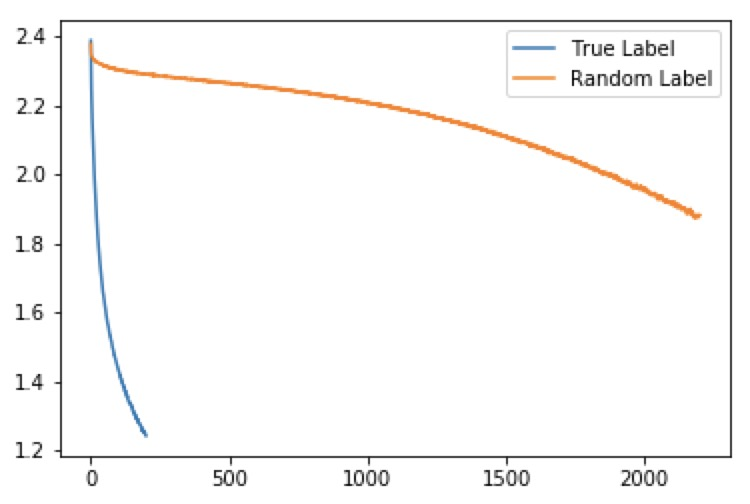
\includegraphics[width=2.5in]{cifar.jpeg}
	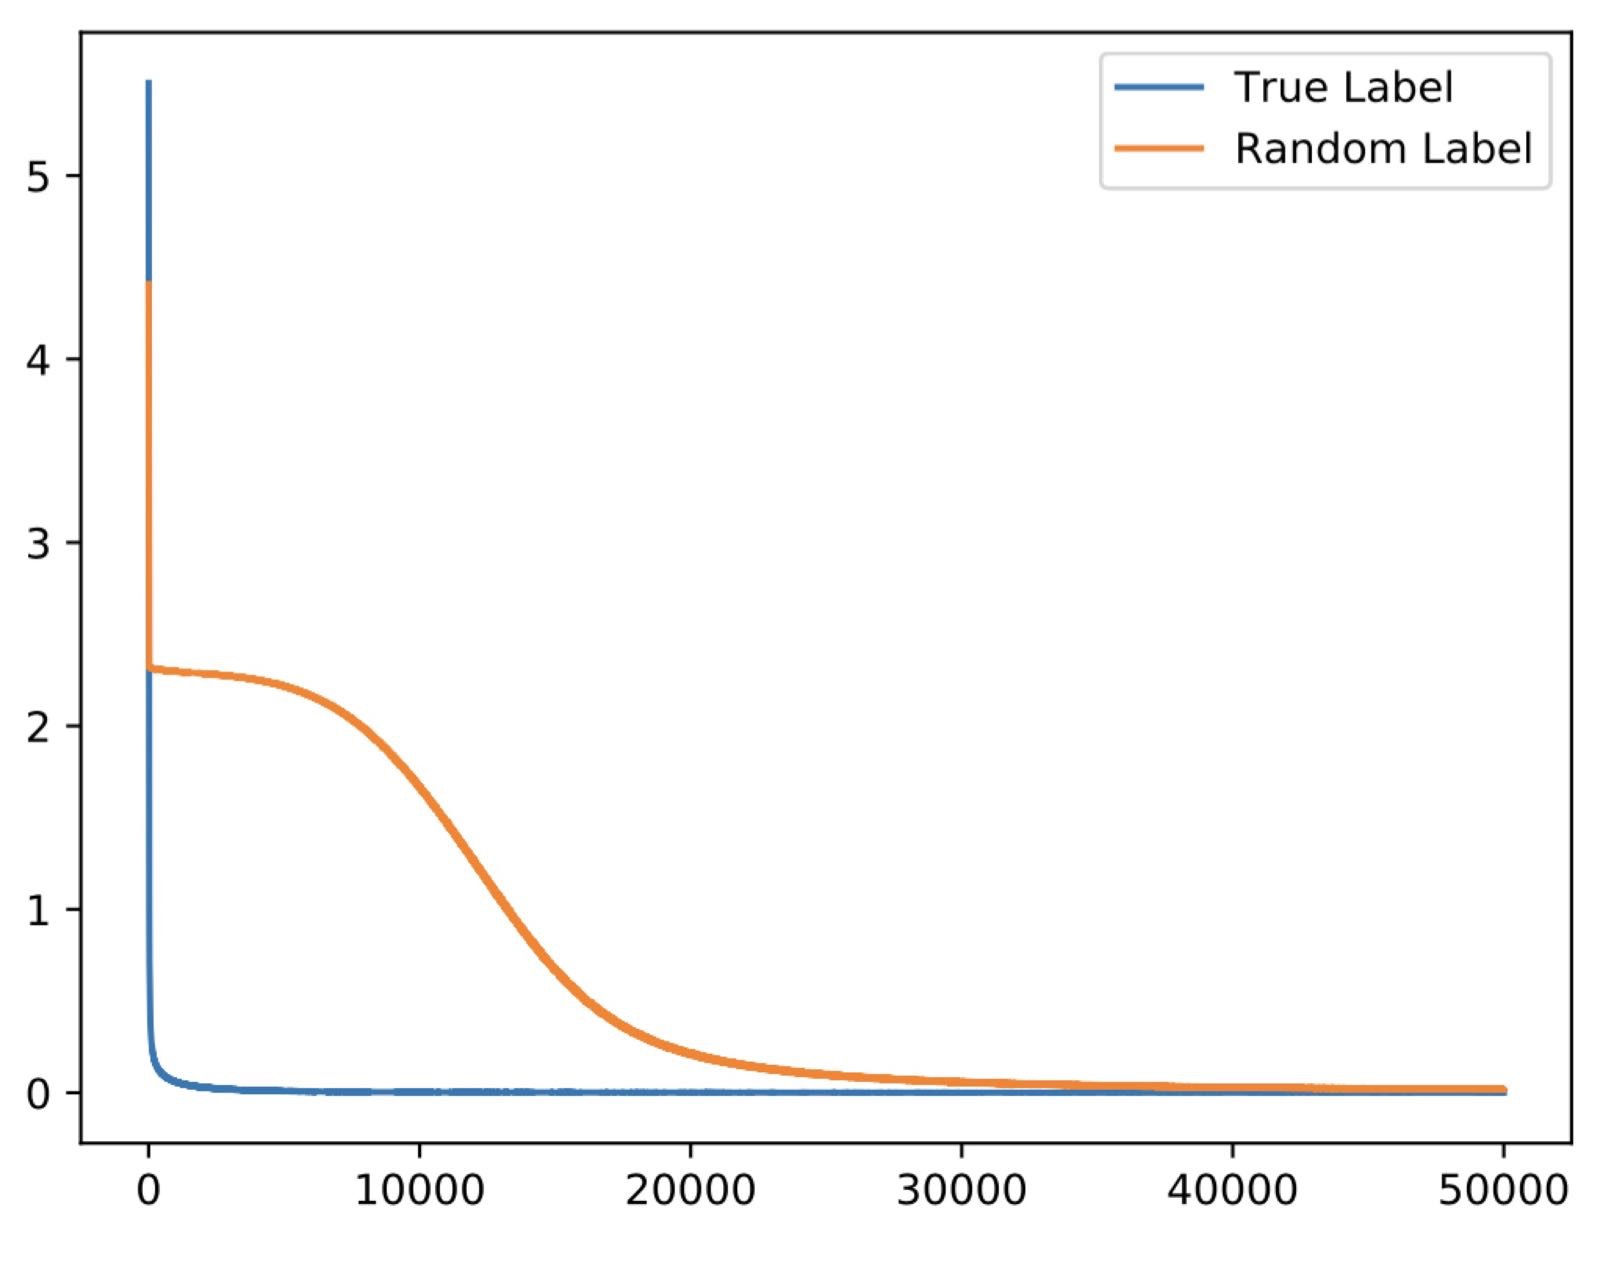
\includegraphics[width=2.5in]{mnist.jpg}
	\caption{Comparison of training the neural network to fit the given label and fit a random labeled dataset using \textbf{gradient descent}. Left hand side is the figure for DenseNet101 training on CIFAR10 dataset and right hand side the one for LeNet5 training on MNIST. It seems that there exists a saddle point around $\log 10$. \textbf{All the loss we evaluate after the last layer is the cross-entropy loss.}}
	\label{saas}
\end{figure}

Figure \ref{saas} shows that the loss of dataset labeled with ground truth drops quickly to zero even when we use the gradient descent algorithm without any noise, which implies that the loss surface in this case is pretty good. However, if we label the data with random choices, the learning curve changes a lot. The loss first quickly drops to a place around $\log 10$ and stops here for a long time. Once the loss leaves $\log 10$, the loss drops faster. This phenomenon suggests that the learning process was going through a saddle point. Repeating the experiment several times, we find that $\log10$ seems a magic number, that all training process starting from a random initialization hits a saddle point near $\log 10$. As the loss function for the last layer output we denote in the experiment is the cross-entropy loss, $\log 10$ is the place where we give a random guess.


\subsection{A Counter Example}

Inspired by the magic number $\log 10$, in this section we give a counter example that there exists a weight, under which condition the random guess is a first order condition but not a global minimum.

In this section, we use the $\ell_2$ loss as the loss function between the target label and the network output. That is to say our objective function is designed as $\argmin_w\mathbb{E}_{(x,y)\sim Dataset}\left\|f_w(x)-y\right\|_2^2$. If the dataset is generated via two independent random variable $x,y$ and $P(y=1)=P(y=-1)=1/2$, then $f_w(x)=0$ for all $x$ is a point that satisfies the first order condition.


\textbf{it seem that this construction is independent of the network structure. It only needs there exist a weight to let the network output is all 0.}

\textbf{write it formally.}

\textbf{I trust you can construct an example. First a weight outputs 0, ex. all the neuron is dead and let several pairs of data is close and half of them is 0 and half of them is 1. next over-paramize(para>data) to construct a smaller value.}

\subsection{Experiments}





\subsection{Data Doesn't Matter}

The success of convolution operator in neural networks is contributes to "the feature of an image depends on the local relationship in an image" and "convolution operator is invariant to translation" in common sense. However, our experiment shows that these factors may not contribute to a nice loss surface. In order to break the translation invariance and local relationship, we randomly permute the pixels in an image and doesn't change the given label. The learning curve is demonstrated in Figure \ref{randomperb}.

\begin{figure}[htp]
	\centering
	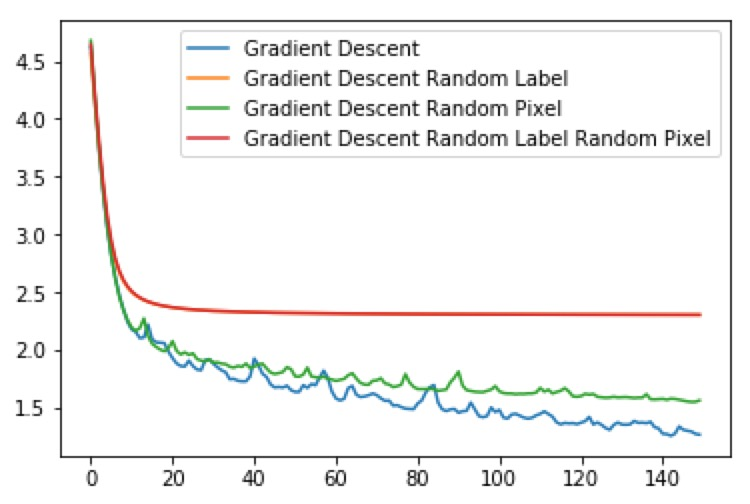
\includegraphics[width=2.5in]{gdrp.jpg}
	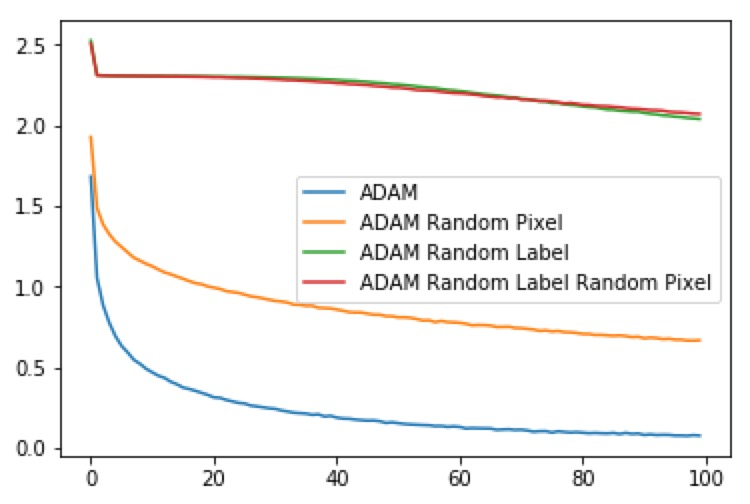
\includegraphics[width=2.5in]{adamrp.jpg}
	\caption{Learning curves for the random permuted dataset and original one. Left hand side is the learning curve of gradient descent algorithm and the right hand side the ADAM algorithm.}
	\label{randomperb}
\end{figure}


\section{Loss surface for one data}

In the next section, we discuss the sufficiency of the cooperation of the data to give a guarantee for a good loss landscape. In this section, we consider the landscape when there is only one data.


\subsection{Vanilla feedforward neural networks}
Consider the loss function of a vanilla feed forward neural network,

$$f(W_1,\cdots,W_n)=\left\|W_n\sigma (W_{n-1}\sigma(W_{n-2}\cdots\sigma(W_1x)))-y\right\|_2^2.$$

Here $x$ is the input data and $y$ is the associated label. $W_i$ is the weight of the $i$-th label and $\sigma$ is the activation function.


$$
\frac{\partial f}{\partial W_i}=\hat\sigma((W_n\sigma (W_{n-1}\sigma(W_{n-2}\cdots\sigma(W_1x)))-y)W_n^t)\cdots
$$

\textbf{check it!} 

Can we give some assumption that leads to for some $i$

$$
\frac{\partial f}{\partial W_i} \ge c|(W_n\sigma (W_{n-1}\sigma(W_{n-2}\cdots\sigma(W_1x)))-y|
$$

\subsection{Deep Residual Networks}

Based on the observation that deep residual network $x_{k+1}=x_{k}+f(x_k)$ can be considered as the forward Euler scheme for an ODE, recent works begin to utilize the ODE to model the deep networks. The learning process can be understood as solving a control problem. There are a lot of work focusing on finding sufficient conditions for the optimal control. In this section, we briefly introduce some of the results and hope to bring some insight for understanding the loss surface of the neural networks.

\textbf{Reachable Set}

\textbf{PMP}

\textbf{Value Function}

This means for a given weight of the last layer, the loss surface seems good. The first order condition(PMP) can imply an optimal control. 

\subsection{Experiments}

\section{Further Directions}

\subsection{Fast Algorithms Escaping Saddle Points}

We also test different algorithms (Momentum SGD, ADAM and AdaDelta) to escape the saddle point around $\log 10$ and the result is demonstrated in Figure \ref{optsadd}. The result shows that both ADAM and AdaDelta can escape from the saddle point and ADAM escapes faster. Can we analyze the escape rate for the AdaDelta? (For ADAM, it has a momentum scheme on gradient which is hard to analyze in the non-convex setting. There are recent papers analyzing AdaGrad in non-convex setting.) There are several factors influencing the speed of accelerating the escaping process:

\begin{itemize}
	\item The adaptive learning rate is large in ADAM and AdaDelta. When stuck in a saddle point, $H_{t+1}=(1-m)H_t+m\hat{g_t}^2$ will become smaller exponentially which means the stepsize increases exponentially.
	\item The adaptive learning rate also estimates the column-wise curvature of the loss surface. If the curvature is estimated correctly, the learning steps will go through the direction associated largest eigenvalue of the Hessian which is the fastest direction to escape the saddle point.
\end{itemize}

\begin{figure}[H]
	\centering
	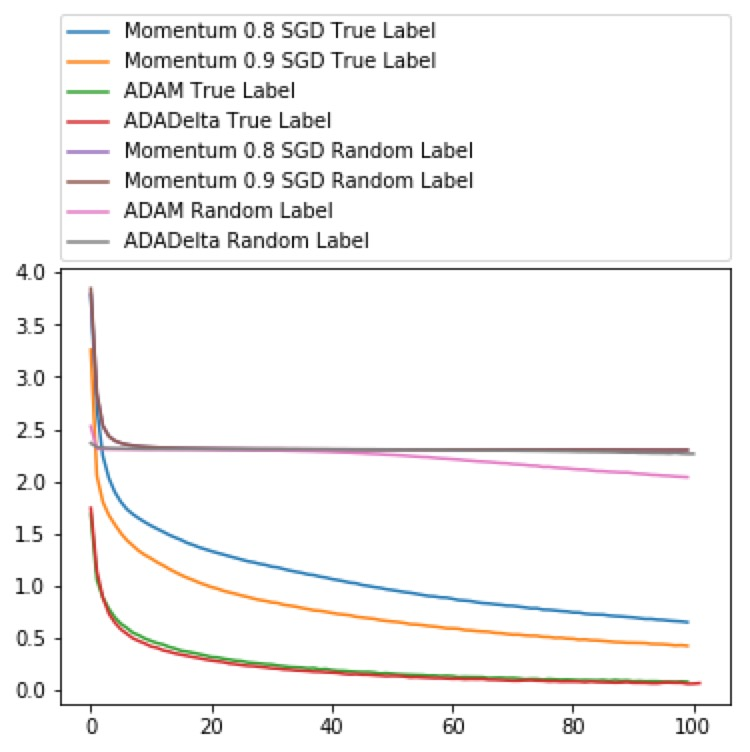
\includegraphics[width=2.5in]{opt.jpg}
	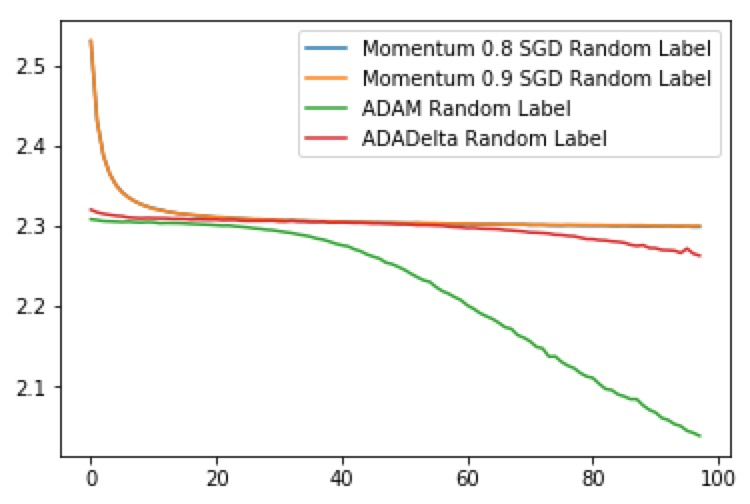
\includegraphics[width=2.5in]{saddle.jpg}
	\caption{Comparison between different optimization algorithm to escape the saddle point around $\log 10$. We test Momentum SGD, ADAM and AdaDelta. ADAM and AdaDelta is able to escape from the saddle point and ADAM performs better. The right hand side figure is a zoom-in version of the first one.}
	\label{optsadd}
\end{figure}

\subsection{Fast Optimization Algorithm Based On The Control Perspective}

There are works showing that we can learn a neural network even if we fixed the last layer's weights. The learning problem turns to a standard control problem. This is natural to apply a \textbf{reinforcement learning} algorithm here. In the previous section, we have introduced that the \textbf{value function} provides a sufficient condition for the control problem. It's natural to use a \textbf{Q-learning} algorithm here to decouple the gradient computation during the back propagation, for the Bellman equation only depends on the previous state the following state.


Another view (It may be another approach) of this kind of decouple learning algorithm is that we can adopt the domain decomposition technique to parallelize the computation of the backward ODE in PMP. Rewrite the adjoint equation in PMP here

$$
\dot p(t) = -p(t)\cdot D_xf(t,x(t),u(t)),p(T)=\nabla \psi(x(T))
$$

Equally, the equation can be written as

$$
\dot p_1(t) = -p_1(t)\cdot D_xf(t,x(t),u(t))|_{t\in[T/2,T]},p_1(T)=\nabla \psi(x(T))$$
$$
\dot p_2(t) = -p_2(t)\cdot D_xf(t,x(t),u(t))|_{t\in[0,T/2]},p_2(T/2)=p_1(T/2)
$$

If we adopt a Gaussian-Seidel like algorithm, we decouple the gradient computation between $[0,T/2]$ and $[T/2,T]$.

\subsection{Proper assumption for label and data assumption}

In our paper, we claim that all the data should cooperate in order to get a good gradient, but how can we define the cooperation of gradients in mathematics.

\subsection{Combine Generalization}


\bibliographystyle{plain}
\bibliography{provably}

\end{document}
